%%*************************************************************************
%% Legal Notice:
%% This code is offered as-is without any warranty either expressed or
%% implied; without even the implied warranty of MERCHANTABILITY or
%% FITNESS FOR A PARTICULAR PURPOSE! 
%% User assumes all risk.
%% In no event shall IEEE or any contributor to this code be liable for
%% any damages or losses, including, but not limited to, incidental,
%% consequential, or any other damages, resulting from the use or misuse
%% of any information contained here.
%%
%% All comments are the opinions of their respective authors and are not
%% necessarily endorsed by the IEEE.
%%
%% This work is distributed under the LaTeX Project Public License (LPPL)
%% ( http://www.latex-project.org/ ) version 1.3, and may be freely used,
%% distributed and modified. A copy of the LPPL, version 1.3, is included
%% in the base LaTeX documentation of all distributions of LaTeX released
%% 2003/12/01 or later.
%% Retain all contribution notices and credits.
%% ** Modified files should be clearly indicated as such, including  **
%% ** renaming them and changing author support contact information. **
%%
%% File list of work: IEEEtran.cls, IEEEtran_HOWTO.pdf, bare_adv.tex,
%%                    bare_conf.tex, bare_jrnl.tex, bare_jrnl_compsoc.tex
%%*************************************************************************

% Note that the a4paper option is mainly intended so that authors in
% countries using A4 can easily print to A4 and see how their papers will
% look in print - the typesetting of the document will not typically be
% affected with changes in paper size (but the bottom and side margins will).
% Use the testflow package mentioned above to verify correct handling of
% both paper sizes by the user's LaTeX system.
%
% Also note that the "draftcls" or "draftclsnofoot", not "draft", option
% should be used if it is desired that the figures are to be displayed in
% draft mode.
%
\documentclass[conference]{IEEEtran}

% *** MISC UTILITY PACKAGES ***
%
\usepackage{ifpdf}
% Heiko Oberdiek's ifpdf.sty is very useful if you need conditional
% compilation based on whether the output is pdf or dvi.
% usage:
% \ifpdf
%   % pdf code
% \else
%   % dvi code
% \fi
% The latest version of ifpdf.sty can be obtained from:
% http://www.ctan.org/tex-archive/macros/latex/contrib/oberdiek/
% Also, note that IEEEtran.cls V1.7 and later provides a builtin
% \ifCLASSINFOpdf conditional that works the same way.
% When switching from latex to pdflatex and vice-versa, the compiler may
% have to be run twice to clear warning/error messages.

\usepackage{blindtext}
\usepackage{placeins}
\usepackage{graphicx}
\usepackage{epstopdf}
\usepackage{hyperref}

% use color package to make todos jump out in text
\usepackage{color}
% macro for todo entries addition
\newcommand{\addtodo}[1]{\textcolor{red}{[[#1]]}}

\definecolor{light-gray}{gray}{0.75}
\newcommand{\dummytext}{\textcolor{light-gray}{\Blindtext}}


% *** CITATION PACKAGES ***
%
%\usepackage{cite}
% cite.sty was written by Donald Arseneau
% V1.6 and later of IEEEtran pre-defines the format of the cite.sty package
% \cite{} output to follow that of IEEE. Loading the cite package will
% result in citation numbers being automatically sorted and properly
% "compressed/ranged". e.g., [1], [9], [2], [7], [5], [6] without using
% cite.sty will become [1], [2], [5]--[7], [9] using cite.sty. cite.sty's
% \cite will automatically add leading space, if needed. Use cite.sty's
% noadjust option (cite.sty V3.8 and later) if you want to turn this off.
% cite.sty is already installed on most LaTeX systems. Be sure and use
% version 4.0 (2003-05-27) and later if using hyperref.sty. cite.sty does
% not currently provide for hyperlinked citations.
% The latest version can be obtained at:
% http://www.ctan.org/tex-archive/macros/latex/contrib/cite/
% The documentation is contained in the cite.sty file itself.






% *** GRAPHICS RELATED PACKAGES ***
%
\ifpdf
  % \usepackage[pdftex]{graphicx}
  % declare the path(s) where your graphic files are
  % \graphicspath{{../pdf/}{../jpeg/}}
  % and their extensions so you won't have to specify these with
  % every instance of \includegraphics
  % \DeclareGraphicsExtensions{.pdf,.jpeg,.png}
\else
  % or other class option (dvipsone, dvipdf, if not using dvips). graphicx
  % will default to the driver specified in the system graphics.cfg if no
  % driver is specified.
  % \usepackage[dvips]{graphicx}
  % declare the path(s) where your graphic files are
  % \graphicspath{{../eps/}}
  % and their extensions so you won't have to specify these with
  % every instance of \includegraphics
  % \DeclareGraphicsExtensions{.eps}
\fi
% graphicx was written by David Carlisle and Sebastian Rahtz. It is
% required if you want graphics, photos, etc. graphicx.sty is already
% installed on most LaTeX systems. The latest version and documentation can
% be obtained at: 
% http://www.ctan.org/tex-archive/macros/latex/required/graphics/
% Another good source of documentation is "Using Imported Graphics in
% LaTeX2e" by Keith Reckdahl which can be found as epslatex.ps or
% epslatex.pdf at: http://www.ctan.org/tex-archive/info/
%
% latex, and pdflatex in dvi mode, support graphics in encapsulated
% postscript (.eps) format. pdflatex in pdf mode supports graphics
% in .pdf, .jpeg, .png and .mps (metapost) formats. Users should ensure
% that all non-photo figures use a vector format (.eps, .pdf, .mps) and
% not a bitmapped formats (.jpeg, .png). IEEE frowns on bitmapped formats
% which can result in "jaggedy"/blurry rendering of lines and letters as
% well as large increases in file sizes.
%
% You can find documentation about the pdfTeX application at:
% http://www.tug.org/applications/pdftex





% *** MATH PACKAGES ***
%
%\usepackage[cmex10]{amsmath}
% A popular package from the American Mathematical Society that provides
% many useful and powerful commands for dealing with mathematics. If using
% it, be sure to load this package with the cmex10 option to ensure that
% only type 1 fonts will utilized at all point sizes. Without this option,
% it is possible that some math symbols, particularly those within
% footnotes, will be rendered in bitmap form which will result in a
% document that can not be IEEE Xplore compliant!
%
% Also, note that the amsmath package sets \interdisplaylinepenalty to 10000
% thus preventing page breaks from occurring within multiline equations. Use:
%\interdisplaylinepenalty=2500
% after loading amsmath to restore such page breaks as IEEEtran.cls normally
% does. amsmath.sty is already installed on most LaTeX systems. The latest
% version and documentation can be obtained at:
% http://www.ctan.org/tex-archive/macros/latex/required/amslatex/math/





% *** SPECIALIZED LIST PACKAGES ***
%
%\usepackage{algorithmic}
% algorithmic.sty was written by Peter Williams and Rogerio Brito.
% This package provides an algorithmic environment fo describing algorithms.
% You can use the algorithmic environment in-text or within a figure
% environment to provide for a floating algorithm. Do NOT use the algorithm
% floating environment provided by algorithm.sty (by the same authors) or
% algorithm2e.sty (by Christophe Fiorio) as IEEE does not use dedicated
% algorithm float types and packages that provide these will not provide
% correct IEEE style captions. The latest version and documentation of
% algorithmic.sty can be obtained at:
% http://www.ctan.org/tex-archive/macros/latex/contrib/algorithms/
% There is also a support site at:
% http://algorithms.berlios.de/index.html
% Also of interest may be the (relatively newer and more customizable)
% algorithmicx.sty package by Szasz Janos:
% http://www.ctan.org/tex-archive/macros/latex/contrib/algorithmicx/




% *** ALIGNMENT PACKAGES ***
%
%\usepackage{array}
% Frank Mittelbach's and David Carlisle's array.sty patches and improves
% the standard LaTeX2e array and tabular environments to provide better
% appearance and additional user controls. As the default LaTeX2e table
% generation code is lacking to the point of almost being broken with
% respect to the quality of the end results, all users are strongly
% advised to use an enhanced (at the very least that provided by array.sty)
% set of table tools. array.sty is already installed on most systems. The
% latest version and documentation can be obtained at:
% http://www.ctan.org/tex-archive/macros/latex/required/tools/


%\usepackage{mdwmath}
%\usepackage{mdwtab}
% Also highly recommended is Mark Wooding's extremely powerful MDW tools,
% especially mdwmath.sty and mdwtab.sty which are used to format equations
% and tables, respectively. The MDWtools set is already installed on most
% LaTeX systems. The lastest version and documentation is available at:
% http://www.ctan.org/tex-archive/macros/latex/contrib/mdwtools/


% IEEEtran contains the IEEEeqnarray family of commands that can be used to
% generate multiline equations as well as matrices, tables, etc., of high
% quality.


%\usepackage{eqparbox}
% Also of notable interest is Scott Pakin's eqparbox package for creating
% (automatically sized) equal width boxes - aka "natural width parboxes".
% Available at:
% http://www.ctan.org/tex-archive/macros/latex/contrib/eqparbox/





% *** SUBFIGURE PACKAGES ***
%\usepackage[tight,footnotesize]{subfigure}
% subfigure.sty was written by Steven Douglas Cochran. This package makes it
% easy to put subfigures in your figures. e.g., "Figure 1a and 1b". For IEEE
% work, it is a good idea to load it with the tight package option to reduce
% the amount of white space around the subfigures. subfigure.sty is already
% installed on most LaTeX systems. The latest version and documentation can
% be obtained at:
% http://www.ctan.org/tex-archive/obsolete/macros/latex/contrib/subfigure/
% subfigure.sty has been superceeded by subfig.sty.



%\usepackage[caption=false]{caption}
%\usepackage[font=footnotesize]{subfig}
% subfig.sty, also written by Steven Douglas Cochran, is the modern
% replacement for subfigure.sty. However, subfig.sty requires and
% automatically loads Axel Sommerfeldt's caption.sty which will override
% IEEEtran.cls handling of captions and this will result in nonIEEE style
% figure/table captions. To prevent this problem, be sure and preload
% caption.sty with its "caption=false" package option. This is will preserve
% IEEEtran.cls handing of captions. Version 1.3 (2005/06/28) and later 
% (recommended due to many improvements over 1.2) of subfig.sty supports
% the caption=false option directly:
%\usepackage[caption=false,font=footnotesize]{subfig}
%
% The latest version and documentation can be obtained at:
% http://www.ctan.org/tex-archive/macros/latex/contrib/subfig/
% The latest version and documentation of caption.sty can be obtained at:
% http://www.ctan.org/tex-archive/macros/latex/contrib/caption/




% *** FLOAT PACKAGES ***
%
%\usepackage{fixltx2e}
% fixltx2e, the successor to the earlier fix2col.sty, was written by
% Frank Mittelbach and David Carlisle. This package corrects a few problems
% in the LaTeX2e kernel, the most notable of which is that in current
% LaTeX2e releases, the ordering of single and double column floats is not
% guaranteed to be preserved. Thus, an unpatched LaTeX2e can allow a
% single column figure to be placed prior to an earlier double column
% figure. The latest version and documentation can be found at:
% http://www.ctan.org/tex-archive/macros/latex/base/



%\usepackage{stfloats}
% stfloats.sty was written by Sigitas Tolusis. This package gives LaTeX2e
% the ability to do double column floats at the bottom of the page as well
% as the top. (e.g., "\begin{figure*}[!b]" is not normally possible in
% LaTeX2e). It also provides a command:
%\fnbelowfloat
% to enable the placement of footnotes below bottom floats (the standard
% LaTeX2e kernel puts them above bottom floats). This is an invasive package
% which rewrites many portions of the LaTeX2e float routines. It may not work
% with other packages that modify the LaTeX2e float routines. The latest
% version and documentation can be obtained at:
% http://www.ctan.org/tex-archive/macros/latex/contrib/sttools/
% Documentation is contained in the stfloats.sty comments as well as in the
% presfull.pdf file. Do not use the stfloats baselinefloat ability as IEEE
% does not allow \baselineskip to stretch. Authors submitting work to the
% IEEE should note that IEEE rarely uses double column equations and
% that authors should try to avoid such use. Do not be tempted to use the
% cuted.sty or midfloat.sty packages (also by Sigitas Tolusis) as IEEE does
% not format its papers in such ways.





% *** PDF, URL AND HYPERLINK PACKAGES ***
%
%\usepackage{url}
% url.sty was written by Donald Arseneau. It provides better support for
% handling and breaking URLs. url.sty is already installed on most LaTeX
% systems. The latest version can be obtained at:
% http://www.ctan.org/tex-archive/macros/latex/contrib/misc/
% Read the url.sty source comments for usage information. Basically,
% \url{my_url_here}.





% *** Do not adjust lengths that control margins, column widths, etc. ***
% *** Do not use packages that alter fonts (such as pslatex).         ***
% There should be no need to do such things with IEEEtran.cls V1.6 and later.
% (Unless specifically asked to do so by the journal or conference you plan
% to submit to, of course. )




% correct bad hyphenation here
\hyphenation{op-tical net-works semi-conduc-tor}


\begin{document}
%
% paper title
% can use linebreaks \\ within to get better formatting as desired
\title{\textbf{\textsc{Dfuzzer}: A D-Bus Service Fuzzing Tool}}

% author names and affiliations
% use a multiple column layout for up to three different
% affiliations
\author{\IEEEauthorblockN{Mat\'{u}\v{s} Marhefka and Petr Muller}
\vspace{5pt}
\IEEEauthorblockA{
	Red Hat Czech\\
	Purky\v{n}ova 99, Brno, Czech Republic\\
	\{mmarhefk\textbar muller\}@redhat.com
}
\vspace{5pt}
\IEEEauthorblockA{
	Faculty of Information Technology\\
	Brno University of Technology\\
	Bo\v{z}et\v{e}chova 2, Brno, Czech Republic}
}

% conference papers do not typically use \thanks and this command
% is locked out in conference mode. If really needed, such as for
% the acknowledgment of grants, issue a \IEEEoverridecommandlockouts
% after \documentclass

% make the title area
\maketitle


\begin{abstract}
We present \textsc{Dfuzzer}, a fully automated tool for fuzz testing
programs communicating via D-Bus. D-Bus is the prevalent modern mechanism for an
inter-process communication in GNU/Linux ecosystem. Programs receiving data over
D-Bus should sanitize the inputs correctly as it may come from any application
having access to the message bus. Unfortunately, it is often not the case as
demonstrated by severe bugs found by the presented fuzzing tool.

\textsc{Dfuzzer} is fully automated: using D-Bus introspection, it is able to
acquire the structure of the parameters expected by the target program. It can
then generate ballast data respecting this structure, so the target program
starts using such data incorrectly if it does not carefully validate it.
We have found numerous bugs in various parts of the GNU/Linux operating system,
including GNOME Shell and systemd. The bugs usually result in crashes, but we
have found other bugs like memory leaks and some data-loss bugs.

We also discuss the software engineering aspects of fuzz testing D-Bus services.
We have met developer opinions that the problems found do not constitute valid bugs, because the D-Bus interface is
actually an internal API. The discussion is interesting by showing that the
D-Bus usage is not a fully mature area of engineering, and the programmers do
not have a shared understanding of its purpose.
\end{abstract}

\begin{keywords}
D-Bus, fuzzer, fuzz testing, automation, pseudo-random data generation, IPC
\end{keywords}

% For peer review papers, you can put extra information on the cover
% page as needed:
% \ifCLASSOPTIONpeerreview
% \begin{center} \bfseries EDICS Category: 3-BBND \end{center}
% \fi
%
% For peerreview papers, this IEEEtran command inserts a page break and
% creates the second title. It will be ignored for other modes.
\IEEEpeerreviewmaketitle



\section{Introduction}
D-Bus is a~binary protocol and~a~message bus system providing applications
a~simple way to~talk to~one another. D-Bus is ``\emph{a~system for~\mbox{inter-process}
communication~(IPC) and~Remote Procedure Calling~(RPC) between
processes running on the same machine and~makes it simple and~reliable to~code
a~`single instance' application or daemon, and~to~launch applications and~daemons
on~demand when their services are needed}''~\cite{dbus}.

Recently, D-Bus has become important part of~almost all GNU/Linux
distributions. There is an increasing number of applications which use it
for~IPC, including key system parts like \textit{systemd} service manager. The
growing importance is witnessed by the recent inclusion of the D-Bus message bus directly into the Linux kernel
upstream.

Applications communicating via D-Bus either provide interfaces which contain callable
methods with~input arguments, or call such methods over
the message bus, providing arguments for them. This means the programs
receiving the data must carefully validate it, because they may originate in
any program having access to the message bus. Unfortunately, this does not seem
to be the usual case, and programs rely on convention and good will of the
callers.

This structure means the D-Bus communicating programs are a good target for
fuzz testing, which is well-suited for detecting bugs stemming from improper
validation of input data. Fuzz testing (or simply fuzzing) is a~well-known type
of~testing~\cite{miller90-fuzz}: it it an automated, brute force, black-box
technique, exploiting the~fact that many bugs in~software are caused
by~handling inputs without applying proper validation routines on~those.
Fuzzing is close to~the~boundary value analysis, where test values are created
to infringe the~boundary of~known good and~bad values.  Fuzz testing has a long
history of being applied in security area~\cite{takanen08-book,sutton07-book},
because the type of bugs it finds often has security implications: improper
validation sometimes means there is a possibility to carefully craft the input
so the program does something useful to the attacker. Outside the security
testing domain, the technique was successfully used for finding bugs in
compilers~\cite{regehr11-compfuzz} and static analyzers~\cite{regehr12-safuzz}.

The advantage of fuzz testing is that the bug detection is easily automated: in
the most basic form, the tool can just send random data as the input of the
program, and the program should not misbehave (usually, crash), but handle the
wrong input gracefully. A testing efficiency can be improved by carefully
crafting the input so it adheres to the protocol expected by the program, but
having random semantics, so it passes the basic validation and penetrates deeper
into the program. For example, if a program expects XML as an input, the fuzzer
will not generate random data, as that would be refused by the most basic XML
parser. Instead, a valid XML containing random elements and their content is
generated, to see how the program validates the input beyond it simply being an
XML.

In this paper, we present \textsc{Dfuzzer}, a fully automated tool for fuzz
testing D-Bus services. \textsc{Dfuzzer} can automatically discover buses,
objects, interfaces and method signatures, so there is no need for difficult
configuration of the tool, although it can easily be focused on just the desired
entities in the system. Careful sanitization of the data received via D-Bus
message is often neglected, and in some cases even thought as unnecessary. One of
the discussed interesting lessons learned by the deployment of
\textsc{Dfuzzer} is the lack of best practices and shared understanding about
D-Bus usage by developers.

The paper is organized as follows. First, we give a brief introduction to D-Bus
message bus infrastructure. Section \ref{sec:C} describes \textsc{Dfuzzer} and compares
it to related tools. We present our results from two deployment stages in
section \ref{sec:D}, where we also discuss the software engineering aspects of
discovered defects and an experience we had during their reporting and repair.

\section{D-Bus message bus}
\label{sec:B}
D-Bus was created to~provide IPC system with a single, unified protocol
and~currently, it is used as default IPC mechanism for~exchanging data between
applications in~desktop environments as for~example GNOME, KDE or Xfce (even
Windows port exists). Besides desktop applications communication it is also used
for~communication between system programs and~user sessions.

\subsection{General Architecture}

D-Bus has both the~system bus daemon (for~events such as ``new hardware device
added'' or ``printer queue changed'') and~the~session bus daemon (for~general
inter-process communication needs among user \mbox{applications}). The~message
bus is built on~top of~a~general one-to-one message passing framework, which
can be used by~any two applications to~communicate directly~(without going
through the~message bus daemon). The~communicating programs are either running
on~one computer, or they communicate through unencrypted TCP/IP socket suitable
for~use behind a~firewall~\cite{dbus}.


D-Bus has several layers:
\begin{itemize}
	\item A~library, \texttt{libdbus}, that allows two applications to~connect
		to~each other and~exchange messages.
	\item A~message bus daemon executable, built on~\texttt{libdbus},
		to which multiple applications can connect. The daemon routes
		messages from~one application to~zero or more others.
	\item Wrapper libraries or bindings based on~particular application frameworks.
\end{itemize}


\begin{figure}[h]
\centering
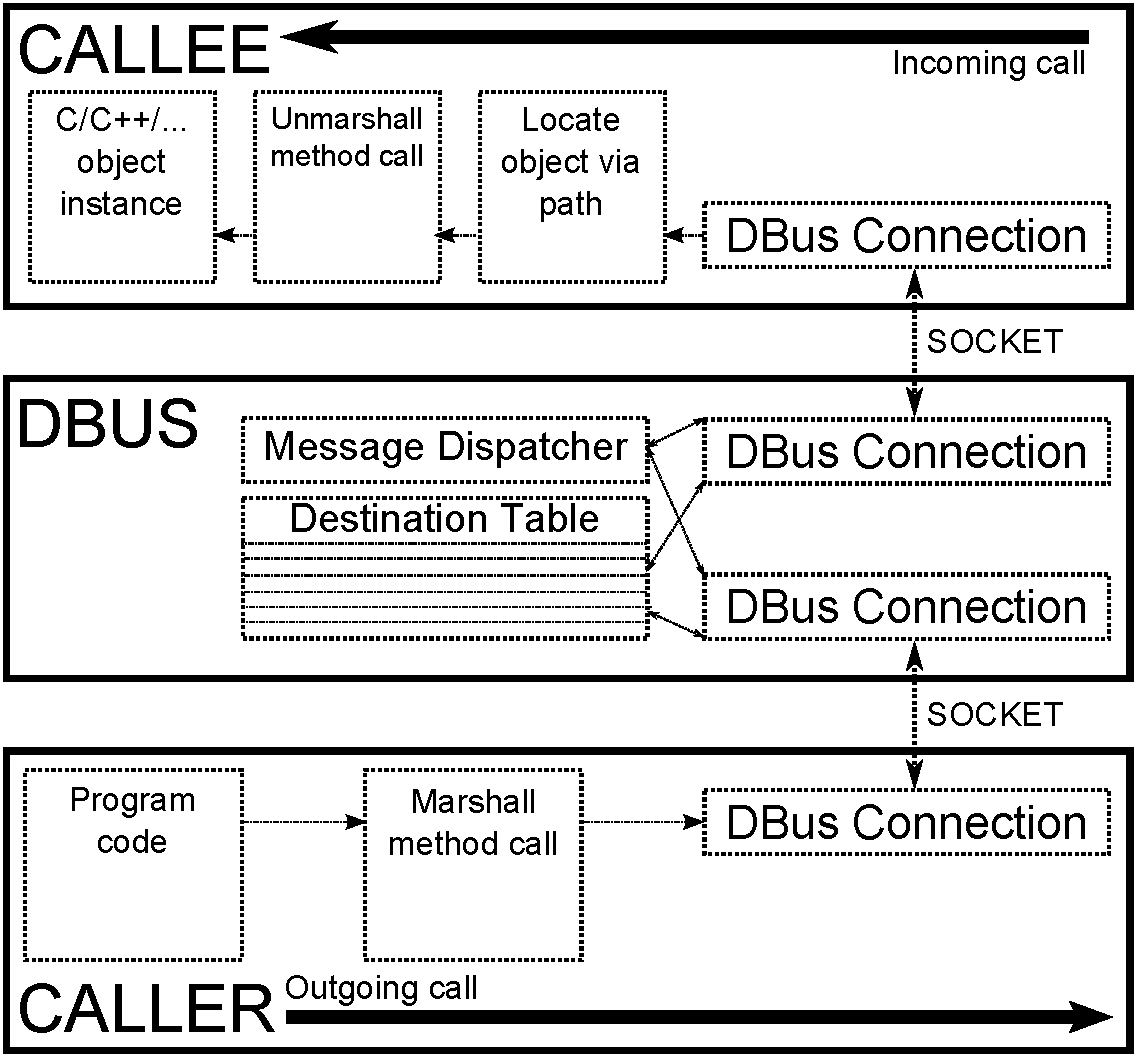
\includegraphics[width=\columnwidth]{dbus_overview.pdf}
\caption{D-Bus overview}
\label{fig:dbus_image}
\end{figure}


D-Bus contains the~bus daemons which act as~routers for~messages. Processes
can connect to~the~bus daemons to~use their routing services as stated
in Figure~\ref{fig:dbus_image}. There are two standard buses:
the~system bus and~the~session bus.


The~system bus is a~global daemon that any application running in~any
context can use as~a~transport router. It is a~single point where applications
can export services that anyone can use. Only one system bus daemon
can be run at a~time within~an~operating system.


The~session bus is the~bus local to~the~current user's session. It is used
for~communication between applications running within the~same X~Window
System\footnote{X~Window is a~system and~a~network protocol that provides
a~basis for~graphical user interfaces.} session. For every login to~X,
a~session bus daemon is started.


D-Bus protocol is binary. Messages consist of~two sections, the~header
and~the~body. The~header contains routing information and~the~type signature
for~the~data. The body contains the~data being sent in~binary format. Each
piece~of~data has a~type code \mbox{associated} with~it and~is packed into the~body
accordingly. Some common types include bytes, 32 and~64 bit integers, doubles,
unix file descriptors and~strings. Common data types can be used to~build more
complex data~types such as arrays, dictionaries or structures.


\subsection{D-Bus Interfaces Provided by Programs}
Messages are sent to~objects. Each object has members of two possible types:
methods and signals.  Methods are operations that can be invoked on~an~object,
with~optional input~(arguments) and~output~(return values).  Signals are
broadcasts from~the~object to~any application on~the~same bus, which registered
that it is interested in~signals emitted by~this object. Signals may contain
a~data payload. Methods and~signals are referred to~by~name.


Each object supports one or more interfaces. An~interface is a~named group
of methods and~signals. D-Bus identifies interfaces with~a~simple namespaced string.
Most bindings to~other programming languages have mapping of~those interface names
directly to~the~appropriate programming language constructs~(C++ virtual classes
for~example).


When each application connects to~the~bus daemon, the~daemon immediately
assigns it a~name, called the unique connection name. Bus daemon ensures that
these unique names are never reused during the~lifetime of~the~bus daemon.


Applications may also own additional well-known names~(also called services),
for example \texttt{org.freedesktop.dfuzzer}. Other applications connected
to~the~same bus daemon could then send messages to~this bus name~(service),
object and interface to~execute method calls.


In~general, the~unique names can be thought of~as IP addresses and~the well-known
names as domain names. So \texttt{org.freedesktop.dfuzzer} might map to~something
like \texttt{:1.396} just as \texttt{google.com} maps to~IP address
\texttt{173.194.35.70}.


Using well-known names~(services) brings one big advantage. When an~application
crashes or exits, the~operating system kernel has a~responsibility to~close
its connection to~the~message bus. As~soon as~the~message bus daemon registers
that an~application disconnected, it sends out notification messages to~all
remaining clients that the~disconnected application names have lost their owner.
This can be used by~other applications to~monitor the~lifetime of~an~application
in~which they are interested or the one with which they are
communicating.

D-Bus methods may accept any number of~arguments and~may return any number
of~values, including none.

Bindings are used to~wrap low-level D-Bus C API calls to~the~higher level
libraries or language constructs. To call a method in the GDBus binding we used
for implementation of \textsc{Dfuzzer}, its name and arguments must be specified. Each
argument of~a~method has its type encoded by a single character. The~signatures
of~arguments are joined to~form the~signature string, similar to~the~format
strings in~\texttt{printf()} function.

\subsection{Object Introspection}

Object introspection is used to~obtain information about object interfaces,
interface methods and~individual method parameters. The call
of~the~\texttt{Introspect} method from
\texttt{org.freedesktop.DBus.Introspectable} interface returns a serialized
form of an introspection of an~object. The example of~introspection
of~the~\texttt{/org/gnome/Shell} object by~calling tool for~working with~D-Bus
objects, \texttt{GDBus}~(with some interfaces omitted for brevity, highlighted
by dots):

{\scriptsize
\begin{verbatim}
<node>
  (...)
  <interface name="org.freedesktop.DBus.Introspectable">
    <method name="Introspect">
      <arg type="s" name="xml_data" direction="out"/>
    </method>
  </interface>
  (...)
  <interface name="org.gnome.Shell">
    <method name="Eval">
      <arg type="s" name="script" direction="in" />
      <arg type="b" name="success" direction="out" />
      <arg type="s" name="result" direction="out" />
    </method>
    <method name="ScreenshotArea">
      <arg type="i" name="x" direction="in" />
      <arg type="i" name="y" direction="in" />
      <arg type="i" name="width" direction="in" />
      <arg type="i" name="height" direction="in" />
      <arg type="b" name="flash" direction="in" />
      <arg type="s" name="filename" direction="in" />
      <arg type="b" name="success" direction="out" />
    </method>
    <method name="Screenshot">
      <arg type="b" name="include_cursor" direction="in" />
      <arg type="b" name="flash" direction="in" />
      <arg type="s" name="filename" direction="in" />
      <arg type="b" name="success" direction="out" />
    </method>
    (...)
    <property type="b" name="OverviewActive"
        access="readwrite" />
    <property type="s" name="ShellVersion"
        access="read" />
  </interface>
  (...)
</node>
\end{verbatim}
}


\noindent
As seen from~object introspection, the~\texttt{/org/gnome/Shell} object has
more interfaces~(object must have at~least one interface). Interfaces has methods
and~signals. Each argument of~a~method is declared with~name, its direction
and~signature string.


%%%%%%%%%%%%%%%%%%%%%%%%%%%%%%%%%%%%%%%%%%%%%%%%%%%%%%%%%%%%%%%%%%%%%%%%
\section{Tool description}
\label{sec:C}
The goal for the presented tool was to fuzz D-Bus clients (the programs using
D-Bus message bus as a communication mean), not the D-Bus message bus itself.
While bringing down the message bus would cause a severe harm to a running
system, it is out of scope for our intentions, as it would require a totally different approach.

\textsc{Dfuzzer} is implemented as a standard D-Bus client. It simply connects
to a message bus (either a session-level or a system-level one) and it calls
remote methods from the interfaces provided on that bus by connected programs.
Connected objects, their interfaces, methods provided by them and their
argument/return value types are discovered automatically by introspection. Any
process connected to a bus and using well-known name can be fuzz tested.

After determining the structure of the interface, the fuzzer starts to craft
random calls of the provided methods. It creates pseudo-random values for
arguments, but it adheres to the expected data type. During these method calls, a target process
is monitored in order to discover an improper reaction to a method call. The
monitor detects if the target process ceases execution (which can indicate a
crash) or significantly raises memory consumption (which may indicate a memory
leak). Ability to detect a failure to respond or target's disconnection from the
message bus is provided directly by the D-Bus infrastructure, so such situations
are trivially detected too.


\subsection{Architecture}
\textsc{Dfuzzer} is divided into three major modules The \emph{random module} is
responsible for~pseudo-random data generation. It can generate pseudo-random
data instances for every primitive data type which can be used in D-Bus method
arguments. The module still has implementation limits in generating complex data
type instances, like structures or arrays.


The~\emph{introspection module} performs an~object
introspection, requesting and processing an introspection file of~a~chosen
object from~the~bus daemon. It also provides the capability to iterate over
discovered interfaces and methods.


The~\emph{fuzz module}, given a method signature, uses the \emph{random} module
to generate the arguments for a method. It then calls the specified method
using the generated arguments. During the call, the target application is
monitored for defect behavior. Failure to respond and disconnection from the
bus conditions are monitored using D-Bus infrastructure. Using
\texttt{/proc/PID/status}\footnote{pid is process identification number} file,
a~tested application process status is monitored in order to confirm that the
target ended itself in some problematic way after disconnecting from~the~bus
daemon. Process status file is also used for~monitoring an~application process
memory usage in order to detect memory leaks after processing a message.


Additionally, the user can specify additional data to be used as arguments
during the testing. This allows to re-use interesting inputs proven to be useful
from different testing rounds. We are planning to add a possibility to mutate
such provided data to discover new, possibly interesting test-cases.

\subsection{Ballast generation} The~\emph{random module} provides functions
for~generation of~all basic data types except arrays, structures
and~dictionaries which were not implemented yet. Besides pseudo-random numbers,
the~\emph{random module} also generates specific boundary values of~number
types in order to perform a directed boundary value testing of target method.
As \textsc{Dfuzzer} uses GDBus binding, the~functions in~the~\emph{random
module} generate only valid UTF-8 strings. Pseudo-random characters which are
used to~fill strings are pruned to~fit the~printable range. Where applicable
(like for strings), a length can be given as a parameter, defining the desired
size of the data instance. This is later used during fuzzing, in order to fuzz
methods with increasingly large arguments as described above.

\subsection{Automated API analysis using introspection}
Before fuzz testing of~a~specified process, object introspection must be done
first. The~interface \texttt{org.freedesktop.DBus.Introspectable} contains
the~\texttt{Introspect} method for obtaining an~XML file containing all
of~the~interfaces and~the~methods of~a~specified process. Returned XML file is
processed into a structure which can be used to~find a~particular interface.
The~\emph{introspection module} which is part of~\textsc{Dfuzzer} encapsulates all
object introspection details and~provides an~interface for~easy iteration
through methods and~their arguments.


Every method argument signature is specified by~its
direction which is either ``out'' (returned argument signature) or
``in''~(accepted argument signature). When an~object introspection of~a~specified
interface is done, \textsc{Dfuzzer} iterates through discovered interface
methods. For~every method, its accepted arguments signatures~(with~direction
``in'') and a~method name are passed to~the~\emph{fuzz module}.

\subsection{Fuzzing the discovered methods} Fuzz testing of~a~method passed
to~the~\emph{fuzz module} takes place in~a~cycle by~calling the method many
times, but with~different arguments.  Before each call of~a~method, its
arguments must be generated first. Arguments are generated by~the~\emph{random
module} according to~method signature. After the call is made, the tool waits
for an answer on message bus (at least the \textit{method return} message is
delivered even for methods with no return value). D-Bus returns a special
constant message in case an error occurred, like a failure to respond or
disconnection from the bus. In such case, the tool can gather more information
about what happened. In addition to built-in information gathering (for crashes
and memory leaks), the user can provide additional scripts for assessing
system integrity. For example, with such additional script, it is possible to
monitor if a fuzzed method call does not result into deletion of some important
file. For the case the target application crashed, \textsc{Dfuzzer} is able to
re-execute it so it can continue with testing.


In~the~case a~tested process crashed or exceeded a~specified memory limit,
a~log is added to a~log file describing a~specified event. A~log file entry is
a~name of~a~method with~its arguments. If some event occurred during testing
a~method, a~log is created within~a~method entry. After a~log header there is
a~message describing an~event which occurred followed by~a~process memory size.
The~last items in~log are the~inputs on~which an~event occurred and~so
the~arguments signatures with~the~corresponding values. An~example
of~the~truncated log file from~fuzz testing the~\emph{GNOME Shell 3.6.3.1}:


{
\footnotesize
\begin{verbatim}
================================================
fuzzing method Eval(s):
end of fuzzing of method 'Eval'
================================================
================================================
fuzzing method ScreenshotArea(i, i, i, i, b, s):
[ScreenshotArea LOG 1]
  process disconnected from D-Bus
  last known process memory size: [289028 kB]
  on input:
  --i-- '2147483647'
  --i-- '2147483647'
  --i-- '2147483647'
  --i-- '-2147483648'
  --b-- 'true'
  --s [length: 27 B]-- '>;VhlC) H-CzF>!550d-49!Nax;'
end of fuzzing of method 'ScreenshotArea'
================================================
================================================
fuzzing method ScreenshotWindow(b, b, b, s):
end of fuzzing of method 'ScreenshotWindow'
================================================
\end{verbatim}
}


The count of calls performed per method depends on types of method arguments.
If only integral arguments are present, a constant count of calls with
different fuzzed arguments is made. The constant is currently hard-coded to one
thousand, but will be likely made configurable in the future.  Whenever an
argument with a notion of length (such as a string) is present, the mechanism
is different in order to find bugs like buffer overflows. Initially, a string
is produced, having both length and content pseudo-random, but length is
limited to be quite small. In later calls, the length limit is increased by a
pseudo-random increment determined from the maximum length the tool is
configured to use. The fuzzing is ended after achieving a limit length, which
can be configured by the user. This way we are able to discover situations
where a program can handle an argument of limited length, and gain insight
about this limit.


\subsection{\textsc{Dfuzzer} usage}
\addtodo{Not that sure about this section. Either remove, or extend.}
\textsc{Dfuzzer} is a command-line tool taking options as arguments for setting-up fuzz
testing of a chosen application. \textsc{Dfuzzer} is fuzz testing only processes
with~well-known names on~the~session bus daemon. This means it needs to~own
only a~unique name within~the~session bus.


By default, \textsc{Dfuzzer} runs in its most general and automated way, where
it automatically discovers all services with well-known names on both message
buses available, and tests everything. Using command-line options, the user can
limit the scope to a certain interface, object or just method, although not to
a single bus.


It is also possible to suppress testing of certain elements in the system,
keeping the ability to automatically discover all available methods. This is
useful during testing sessions, because some interface interactions can
destroy a running system by shutting it down, suspending it or disconnect it
from the network.

\subsection{Limitations and further plans}
The tool, in its current state, has several limitations. It is not able to generate some possible invalid D-Bus
messages, like using invalid UTF-8 strings as arguments. This limitation is
caused by our usage of the GDBus binding library, which does basic data type
sanitization. Thus, it is not possible to send invalid D-Bus messages this way,
although a program not using this binding would be able to do so, in theory. We
do not see this limitation as very serious one, as it seems sufficient to
generate valid D-Bus messages to create problems for programs. To explore
program reactions on invalid D-Bus messages, it should be possible to either
circumvent the binding totally, or at least modify the binding so it omits the
validation.


The second limitation, planned to be removed by further development, is the
inability to generate pseudo-random arguments of more complex types, such as 
structures, arrays and~dictionaries. This is just an implementation deficiency
and we expect the rectification to bring a better bug detection ability. 


The final serious limitation is the current inability to create fuzzed D-Bus
signals to test programs listening for these. \textsc{Dfuzzer} can currently
test just D-Bus method calls. Because we see the programs handling signals as
another interesting input vector, we also plan to rectify this limitation by
further work.


There are some enhancements planned for the future development of
\textsc{Dfuzzer}. First enhancement planned is the ability to minimize the
testcase in order to discover which parameter value (or which combination of
parameter) is really causing the failure. Second enhancement is to improve the
bug finding capabilities by the ability to drive the tested service into certain
state using D-Bus messages with known and valid messages.


\subsection{Project details}
\textsc{Dfuzzer} is written in C language. The source code is publicly
available\footnote{\url{https://github.com/matusmarhefka/dfuzzer}} under the GNU
GPLv3 license. The initial work on the project was performed as a part of a bachelor
thesis in cooperation of Red Hat Czech and Faculty of Information Technology, Brno
University of Technology.

The tool uses two important external libraries: \texttt{libffi} and
\texttt{GLib2}. \texttt{Libffi} is a foreign function interface library. It
provides a pointer to a function that can accept and decode any combination of
arguments defined at runtime.  \texttt{GLib2} is the low-level core library
which provides data structure handling for C, portability wrappers, and
interfaces for runtime functionality such as an event loop, threads, dynamic
loading and an object system.  \texttt{GLib2} also provides GDBus bindings, so
applications do not have to be written in low-level D-Bus C library and instead
use the high-level advantages of GDBus binding and data types from
\texttt{Glib2}.

\subsection{Related work}
Our motivation for creating the tool was the fact there is no general,
well described fuzzer already existing. The only comparable tool available is
\texttt{dbusfuzz.py}~\footnote{\url{https://chromium.googlesource.com/chromiumos/platform/dbusfuzz/+/master/dbusfuzz.py}},
implemented as part of the Chromium project by Google. All reasoning about this
tool had to be made from its code, as there is no documentation or publication
available. In purpose, it seems to be similar to that of \textsc{Dfuzzer}. It
also targets D-Bus services. The comparison of the main features of these two
tools is present in Table \ref{tab:differences}. 

\FloatBarrier
\begin{table}[!h]
\caption{Differences between Dfuzzer and Dbusfuzz}
\label{tab:differences}
\begin{center}
	\begin{tabular}{|l|c|c|}
	\hline
	\textbf{Property} & \textbf{Dfuzzer} & \textbf{dbusfuzz.py} \\ \hline \hline
	Language & C with GLib2 & Python \\ \hline
	Fuzzing approach & generation & mutation \\ \hline
	Interface discovery & yes & no \\ \hline
	Continue on crash & yes & no \\ \hline
	Configurability & bus, interface & bus, interface  \\
	 & object, method & object, method \\
	 & strings arguments & all arguments \\ \hline
	Error messages & Human readable errors & Python tracebacks \\ \hline
 
	\end{tabular}
\end{center}
\end{table}
\FloatBarrier

It mostly seems that \texttt{dbusfuzz.py} is designed to be used programatically
(as it consumes YAML as input and emits failures as Python tracebacks), so it is basically a functional subset of \textsc{Dfuzzer}. The main advantage
of \textsc{Dfuzzer} is the ability to automatically discover interfaces using
introspection, whereas \texttt{dbusfuzz.py} needs a test plan specified in YAML
input.
It is also less robust and terminates on first defect found. \textsc{Dfuzzer} can
continue testing after finding a defect by re-executing the target. The tools
also differ in fuzzing approach. \textsc{Dfuzzer} generates data entirely
pseudo-randomly. \texttt{dbusfuzz.py} uses a mutation approach, where it mutates
values given initially in the test plan.


BendyBus\footnote{\url{http://tecnocode.co.uk/2012/01/19/all-aboard-the-bendy-bus/}}
is another tool for fuzz testing applications. Opposed to \textsc{Dfuzzer},
which tests D-Bus services (which are similar to servers), BendyBus targets
users/clients of these services. BendyBus simulates a D-Bus service by mocking
its interfaces and methods, and responds to clients with fuzzed messages. It
targets the client applications and so its purpose is different from the
purpose of \textsc{Dfuzzer}. In full testing of whole D-Bus eco-system in a
operating system distribution, \textsc{Dfuzzer} and BendyBus might complement each other nicely.

\section{Results}
\label{sec:D}
We present two sets of experiment results of the tool. First experiment stage
was to determine the ability of the tool to find bugs in real code and the
usefulness of the provided defect reports. After the tool was mature enough and
the ability to find real bugs was confirmed, we have adopted it to perform a
testing campaign on the Red Hat Enterprise Linux operating system distribution.
 
\subsection{Experiments on selected packages}
The initial testing focused on the tool's ability to detect crashes, memory
leaks and also exceptions from D-Bus daemons. We have tested this ability
on a crafted D-Bus service exhibiting all this erroneous behavior.
To confirm that \textsc{Dfuzzer} is able to detect these issues even in
real-world software, we have selected three mature components of the GNU/Linux
desktop for further testing: GNOME Shell, IMSetting and Evince. 

GNOME Shell is the~core user interface of~the~GNOME desktop environment
providing basic functionality like switching between windows and~launching
applications. We have chosen GNOME Shell as it is a prominent user of D-Bus
communication, a key part of the desktop, and it was under heavy development
at the time.
By testing its D-Bus interfaces we immediately found it does not validate its
input data, and managed to crash not only the GNOME Shell process, but also
(with a different input) whole GNOME desktop session instance.

Both these bugs were reported to the GNOME Bugzilla\footnote{
\url{https://bugzilla.gnome.org/show_bug.cgi?id=699752}}, and we met
some resistance about whether these crashes actually constitute real bugs, because
the D-Bus interface is intended to be used only by certain GNOME components which behave
nicely. As we encountered more such discussions in further bug reporting, we
discuss this situation in a separate section below, because we think it is an
interesting software engineering issue on its own.

The next target selected for testing was IMSettings, a~framework handling input
method settings in a way that any change is propagated immediately and takes
effect without~restarting applications and~a~desktop session. This application
was chosen because it is processing inputs from different human languages.
We discovered IMSettings does not validate inputs as well as we found 6 bugs
including three different inputs crashing the program. We have also found few
potential memory leaks. The biggest leak caused memory usage to raise 146.6
times, from the initial usage of 748 kB to 107 MB.

Evince, which is a~document viewer for~multiple document formats, was tested
with \textsc{Dfuzzer} as well. We have not detected any bugs in its D-Bus interfaces.

\subsection{Distribution-wide deployment}
When the \textsc{Dfuzzer} implementation and functionality reached our requirements
and stability, it was used to perform a testing campaign on a Red Hat Enterprise
Linux distribution of GNU/Linux. The target was to test all D-Bus services in
the full installation of the operating system, listening on either a system or a
session bus daemon. The total was 32 services provided by different components
in the system. Out of these 32 services, we have found at least one test failure
in 16 of them. In total, we discovered 31 different methods were not handling an
input correctly, usually crashing or increasing memory consumption in a
significant way.

The most critical bug found was a removal of a root account, occurring during
fuzz testing a service provided by the \emph{accountsservice} package. The fuzzer
ran with sufficient privileges to do this, so although this is not a security
issue, it is still serious enough as the D-Bus vector circumvents the protection
the appropriate client tool for account management has for this special case.

\FloatBarrier
\begin{table}[!h]
\caption{Bugs found in RHEL packages}
\label{tab:foundbugs}
\begin{center}
	\begin{tabular}{|l|c|l|}
	\hline
	\textbf{Package} & \textbf{Bug count} & \textbf{Bug types} \\ \hline \hline
	accountsservice & 5 & removal of root, memory leaks \\ \hline
	systemd & 2 & crashes \\ \hline
	avahi & 2 & crashes \\ \hline
	colord & 2 & crashes, memory leaks \\ \hline
	firewalld & 3 & memory leaks \\ \hline
	abrt & 1 & memory leaks \\ \hline
	gdm & 1 & memory leaks \\ \hline
	gnome-shell & 1 & crashes \\ \hline
	gnome-session & 1 & crashes \\ \hline
	gnome-desktop3 & 1 & crashes \\ \hline
	gjs & 1 & crashes \\ \hline
	tracker & 1 & memory leaks \\ \hline
	imsettings & 6 & crashes, memory leaks \\ \hline
	kde-workspace & 1 & crashes \\ \hline
	kde-runtime & 2 & crashes, memory leaks \\ \hline
	polkit-kde & 1 & memory leaks \\ \hline
	\textbf{Bugs total} & \textbf{31} & \\ \hline 
	\end{tabular}
\end{center}
\end{table}
\FloatBarrier

\subsection{Software development implications}
In this section, we discuss an interesting finding about the
nature of defects discovered by \textsc{Dfuzzer}. In some cases, we met an opposition
from the affected project developers, commenting that these reported issues are
not real bugs. Arguments for these claims were stemming from an
opinion that the D-Bus interface of the program is supposed to be an internal API, and
therefore not necessary to be robust and handle any input. In other cases, the
findings were acknowledged as bugs and promptly fixed. In our opinion, this
witnesses the adoption of D-Bus communication usage in modern GNU/Linux
desktop is not mature enough to have widely accepted best practices. The
decision about the realistic need to sanitize inputs received via D-Bus is usually not done at all, but depends on the habit and preference of certain developer.


We argue that we cannot speak of an internal API for applications receiving
their inputs via D-Bus, especially not the crucial parts of the running system
like GNOME Shell or systemd. Not sanitizing inputs means reliance that the
other side of the communication behaves nicely and provides just the expected
range of arguments. The problem is that any program, not just the one expected,
having access to the appropriate message bus (so these problems generally does
not have severe security implications, as there is no way to elevate privileges
this way, just create a denial of service locally in a context where you may
terminate the service directly) may attempt to communicate with the other
program listening on that bus.
These programs may, by poor programming or by malice, supply any value
permitted by the expected data type as an argument.  When the receiving program
does not do proper validation, a well-known situation happens where dirty data
are processed by the program and anything may happen, from a program simply
crashing to unintended and dangerous operations, like the described case of a
root account removal. We argue that it should not be this easy to bring down
key parts of a running system simply by passing them garbage via publicly
facing interface.


Reporting the defects found by \textsc{Dfuzzer} had a useful effect of bringing
attention to the D-Bus messages being a standard input vector, which may need to
be sanitized prior to using. With more testing and new defects reported, the
discussions will likely lead to the creation of best practices and shared
understanding of D-Bus usage principles.


\section{Conclusion}
In this paper, we presented \textsc{Dfuzzer}, a tool for fuzz testing
applications receiving their input via D-Bus message bus, an emerging
communication mechanism for modern GNU/Linux desktop systems. Applications
receiving data through this message bus, in our opinion, provide a semi-public
interface to any program running on the system, and therefore should validate
received data in the same way as they should validate any other generally
untrusted input. In our deployment of the tool, we found that many programs are
not properly doing this, resulting in crashes, memory leaks and unintended
behavior defects. \textsc{Dfuzzer} is able to expose these bugs.  In the
future, we plan to extend \textsc{Dfuzzer} to be able to generate even data of
more complex data types. We also plan to enhance the tool to fuzz D-Bus
signals, exposing the additional input vectors of programs using D-Bus to
unexpected data.  \textsc{Dfuzzer} is fully automated, which allows an easy
deployment and usage.  We plan to deploy it for testing all programs in the
Fedora GNU/Linux distribution, which use D-Bus for communication.


% trigger a \newpage just before the given reference
% number - used to balance the columns on the last page
% adjust value as needed - may need to be readjusted if
% the document is modified later
%\IEEEtriggeratref{8}
% The "triggered" command can be changed if desired:
%\IEEEtriggercmd{\enlargethispage{-5in}}

% references section

% can use a bibliography generated by BibTeX as a .bbl file
% BibTeX documentation can be easily obtained at:
% http://www.ctan.org/tex-archive/biblio/bibtex/contrib/doc/
% The IEEEtran BibTeX style support page is at:
% http://www.michaelshell.org/tex/ieeetran/bibtex/
%\bibliographystyle{IEEEtran}
% argument is your BibTeX string definitions and bibliography database(s)
%\bibliography{IEEEabrv,../bib/paper}
%
% <OR> manually copy in the resultant .bbl file
% set second argument of \begin to the number of references
% (used to reserve space for the reference number labels box)
\begin{thebibliography}{1}

\bibitem{sutton07-book}
Michael~Sutton, Adam~Greene and Pedram~Amini. \emph{Fuzzing: Brute Force
Vulnerability Discovery}, Addison-Wesley Professional, 2007.

\bibitem{takanen08-book}
Ari~Takanen and Jared~DeMott and Charlie~Miller. \emph{Fuzzing for~Software
Security Testing and~Quality Assurance}, Artech House Print on~Demand, 2008.

\bibitem{dbus}
Red Hat and the community. \emph{Software/dbus [online]}, freedesktop.org,
2012-08-24 [cit. 2014-10-01],
\url{http://www.freedesktop.org/wiki/Software/dbus}

\bibitem{regehr11-compfuzz}
Xuejun Yang, Yang Chen, Eric Eide, and John Regehr. \emph{Finding and
Understanding Bugs in C Compilers}. In Proceedings of 32nd ACM SIGPLAN
Conference on Programming Language Design and Implementation (PLDI 2011). San Jose, CA, USA, June 2011.

\bibitem{regehr12-safuzz}
Pascal Cuoq, Benjamin Monate, Anne Pacalet, Virgile Prevosto, John Regehr, Boris
Yakobowski, and Xuejun Yang. \emph{Testing static analyzers with randomly
generated programs}. Short paper in Proceedings of the 4th NASA Formal Methods Symposium (NFM 2012). Norfolk, Virginia, USA, April 2012.

\bibitem{miller90-fuzz}
B.P. Miller, L. Fredriksen, and B. So. \emph{An Empirical
Study of the Reliability of UNIX Utilities}. Communications of the ACM 33, 12
(December 1990)

\end{thebibliography}

\appendix
\section{Live demonstration plan}
\begin{itemize}
	\item D-Bus introspection
		\begin{itemize}
			\item Overview of running D-Bus infrastructure
			\item Details of running services
			\item Use DFuzzer's ability to discover different interfaces, objects and
			methods
		\end{itemize}
	\item Demonstrate fuzz testing of the D-Bus service
		\begin{itemize}
			\item Run in fully automated mode, discovering every testable method
			\item Show limiting to certain elements on the bus
			\item Show detection of a service crashing on an input
			\item Show detection of a service leaking memory
		\end{itemize}
	\item Demonstrate detection scripts
		\begin{itemize}
			\item Enhance DFuzzer with custom detection scriptb
			\item Show this enhancement in action
		\end{itemize}
\end{itemize}
% that's all folks
\end{document}
